\documentclass{beamer}
\usepackage{amsmath}
\usepackage[latin1]{inputenc}
\usefonttheme[onlylarge]{structurebold}
\setbeamerfont*{frametitle}{size=\normalsize,series=\bfseries}
\setbeamertemplate{navigation symbols}{}
\usetheme{Goettingen}
\defbeamertemplate{itemize item}{checkbox}{\Square}
\defbeamertemplate{itemize item}{checked}{\Square\llap\CheckmarkBold}

\title[Lab Meeting V]{Lab Meeting V}
\author{Carles Boix}
\begin{document}

\begin{frame}
    \begin{center}
        {\large \textsc{Last Two Weeks (11/25 and 12/02):}}
    \end{center}
    \begin{minipage}[ht!]{.48\textwidth}
          \begin{figure}[ht!]
            \centering
            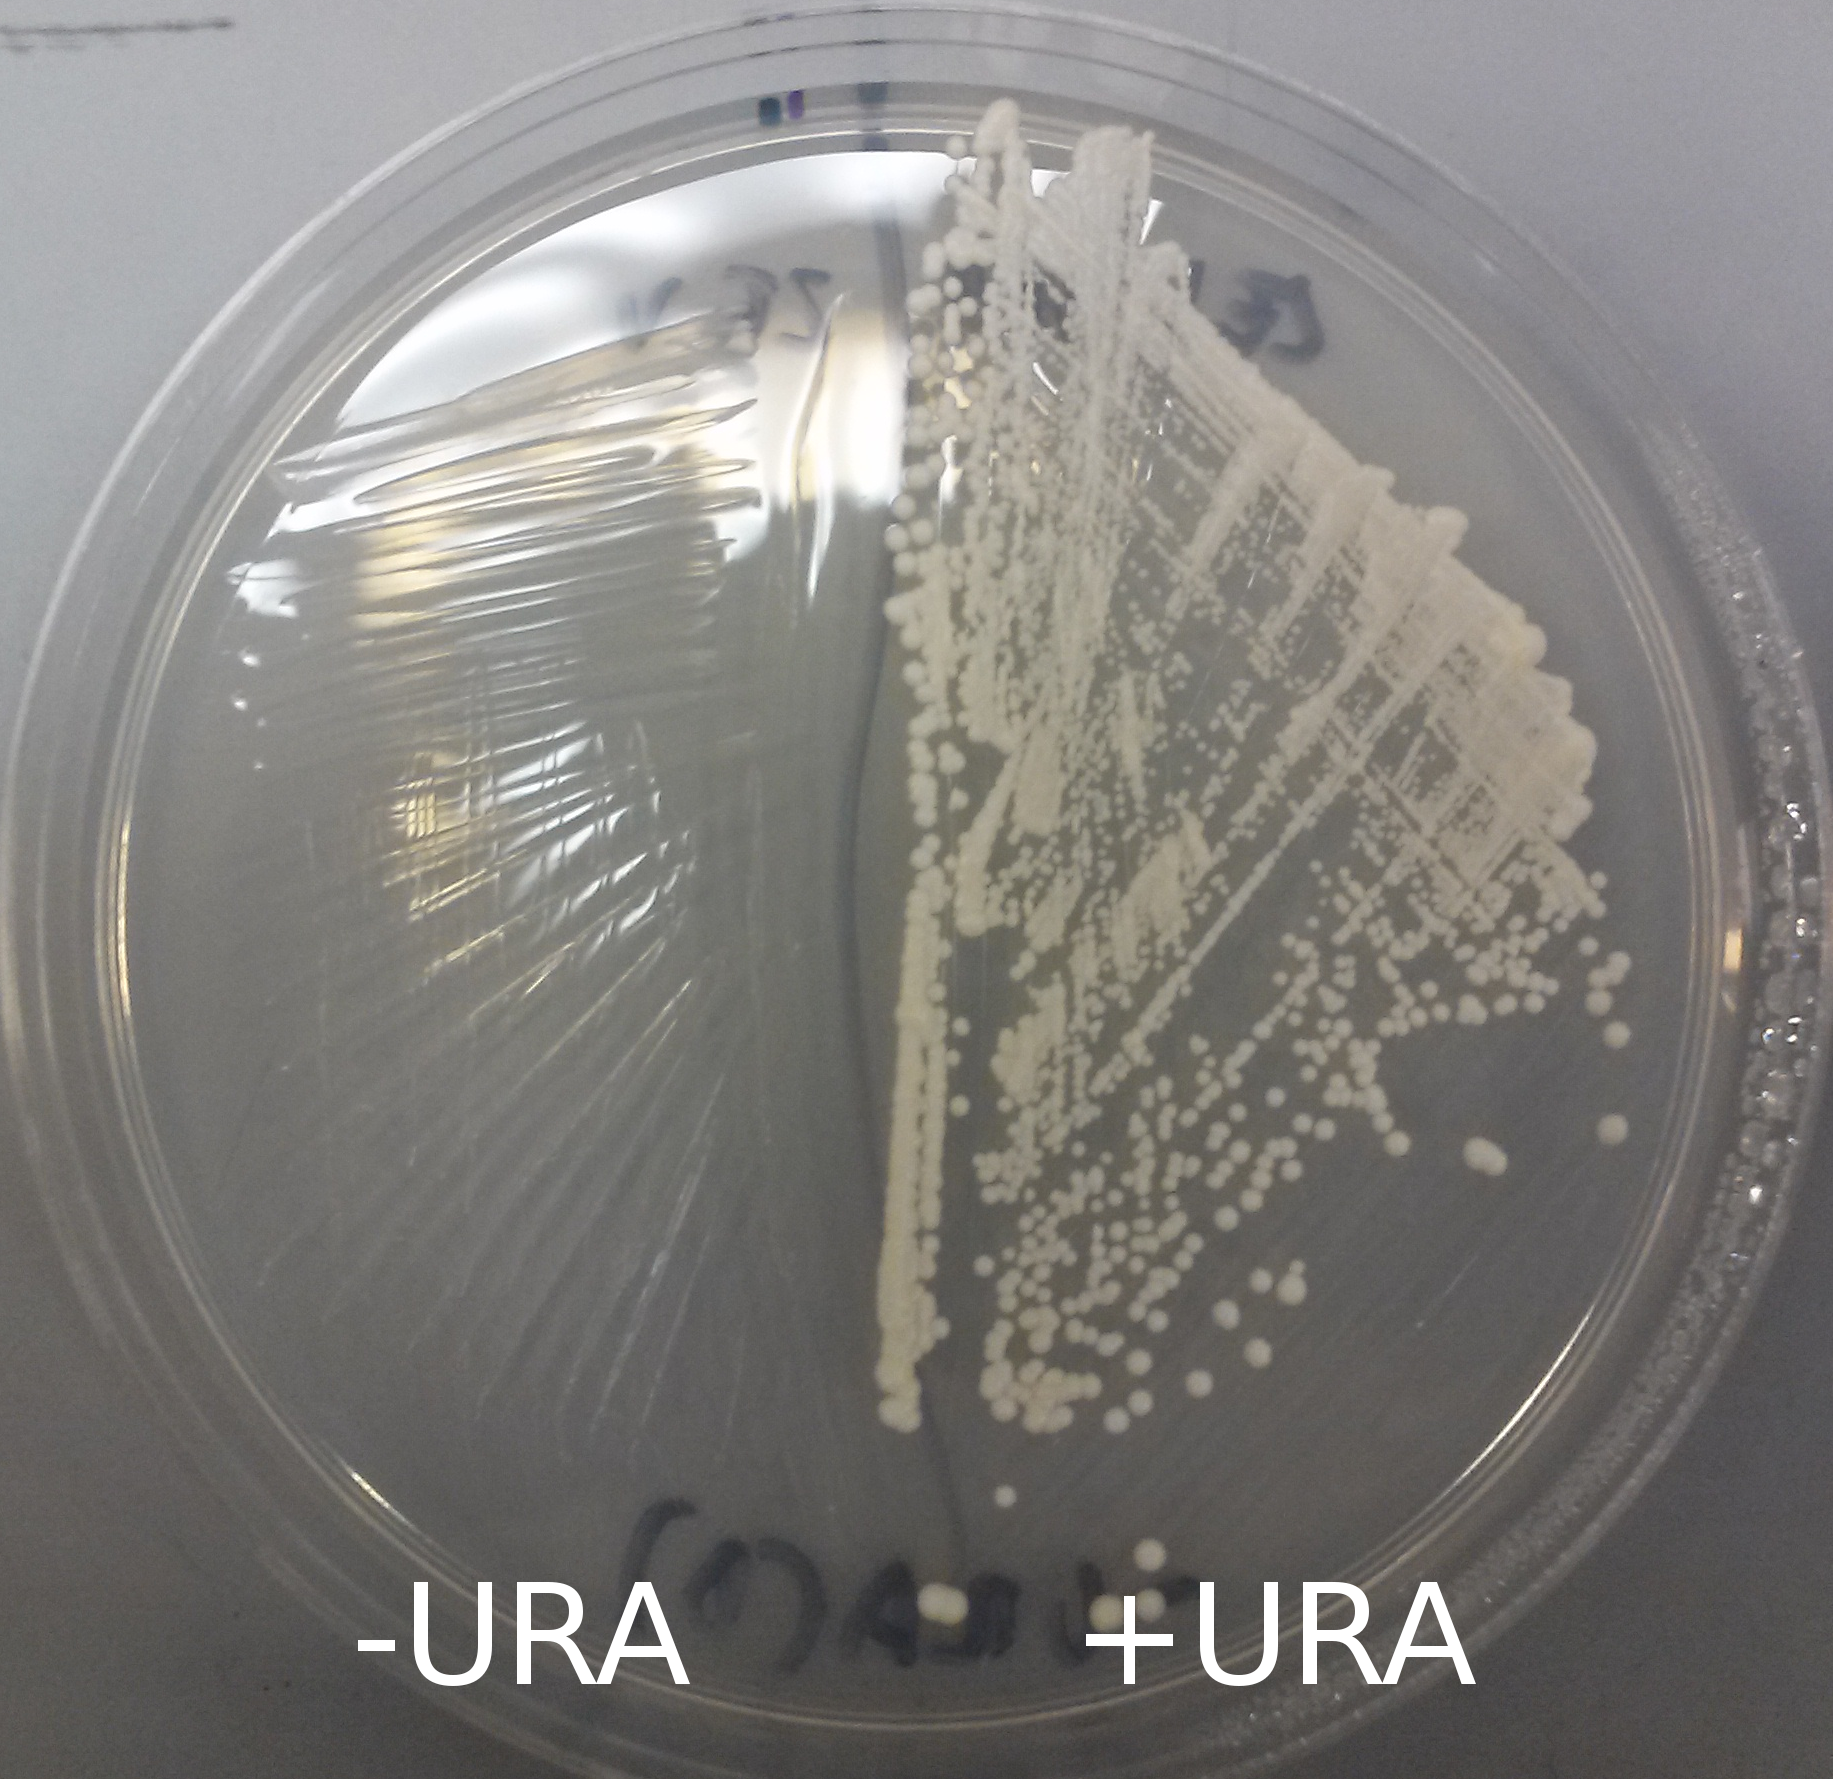
\includegraphics[width=.9\textwidth]{URAtest.png}
            \caption{Test of SC -URA plate}
            \label{fig:pcr}
        \end{figure}
    \end{minipage}
    \hfill
    \begin{minipage}[ht!]{.48\textwidth}
         \begin{figure}[ht!]
            \centering
            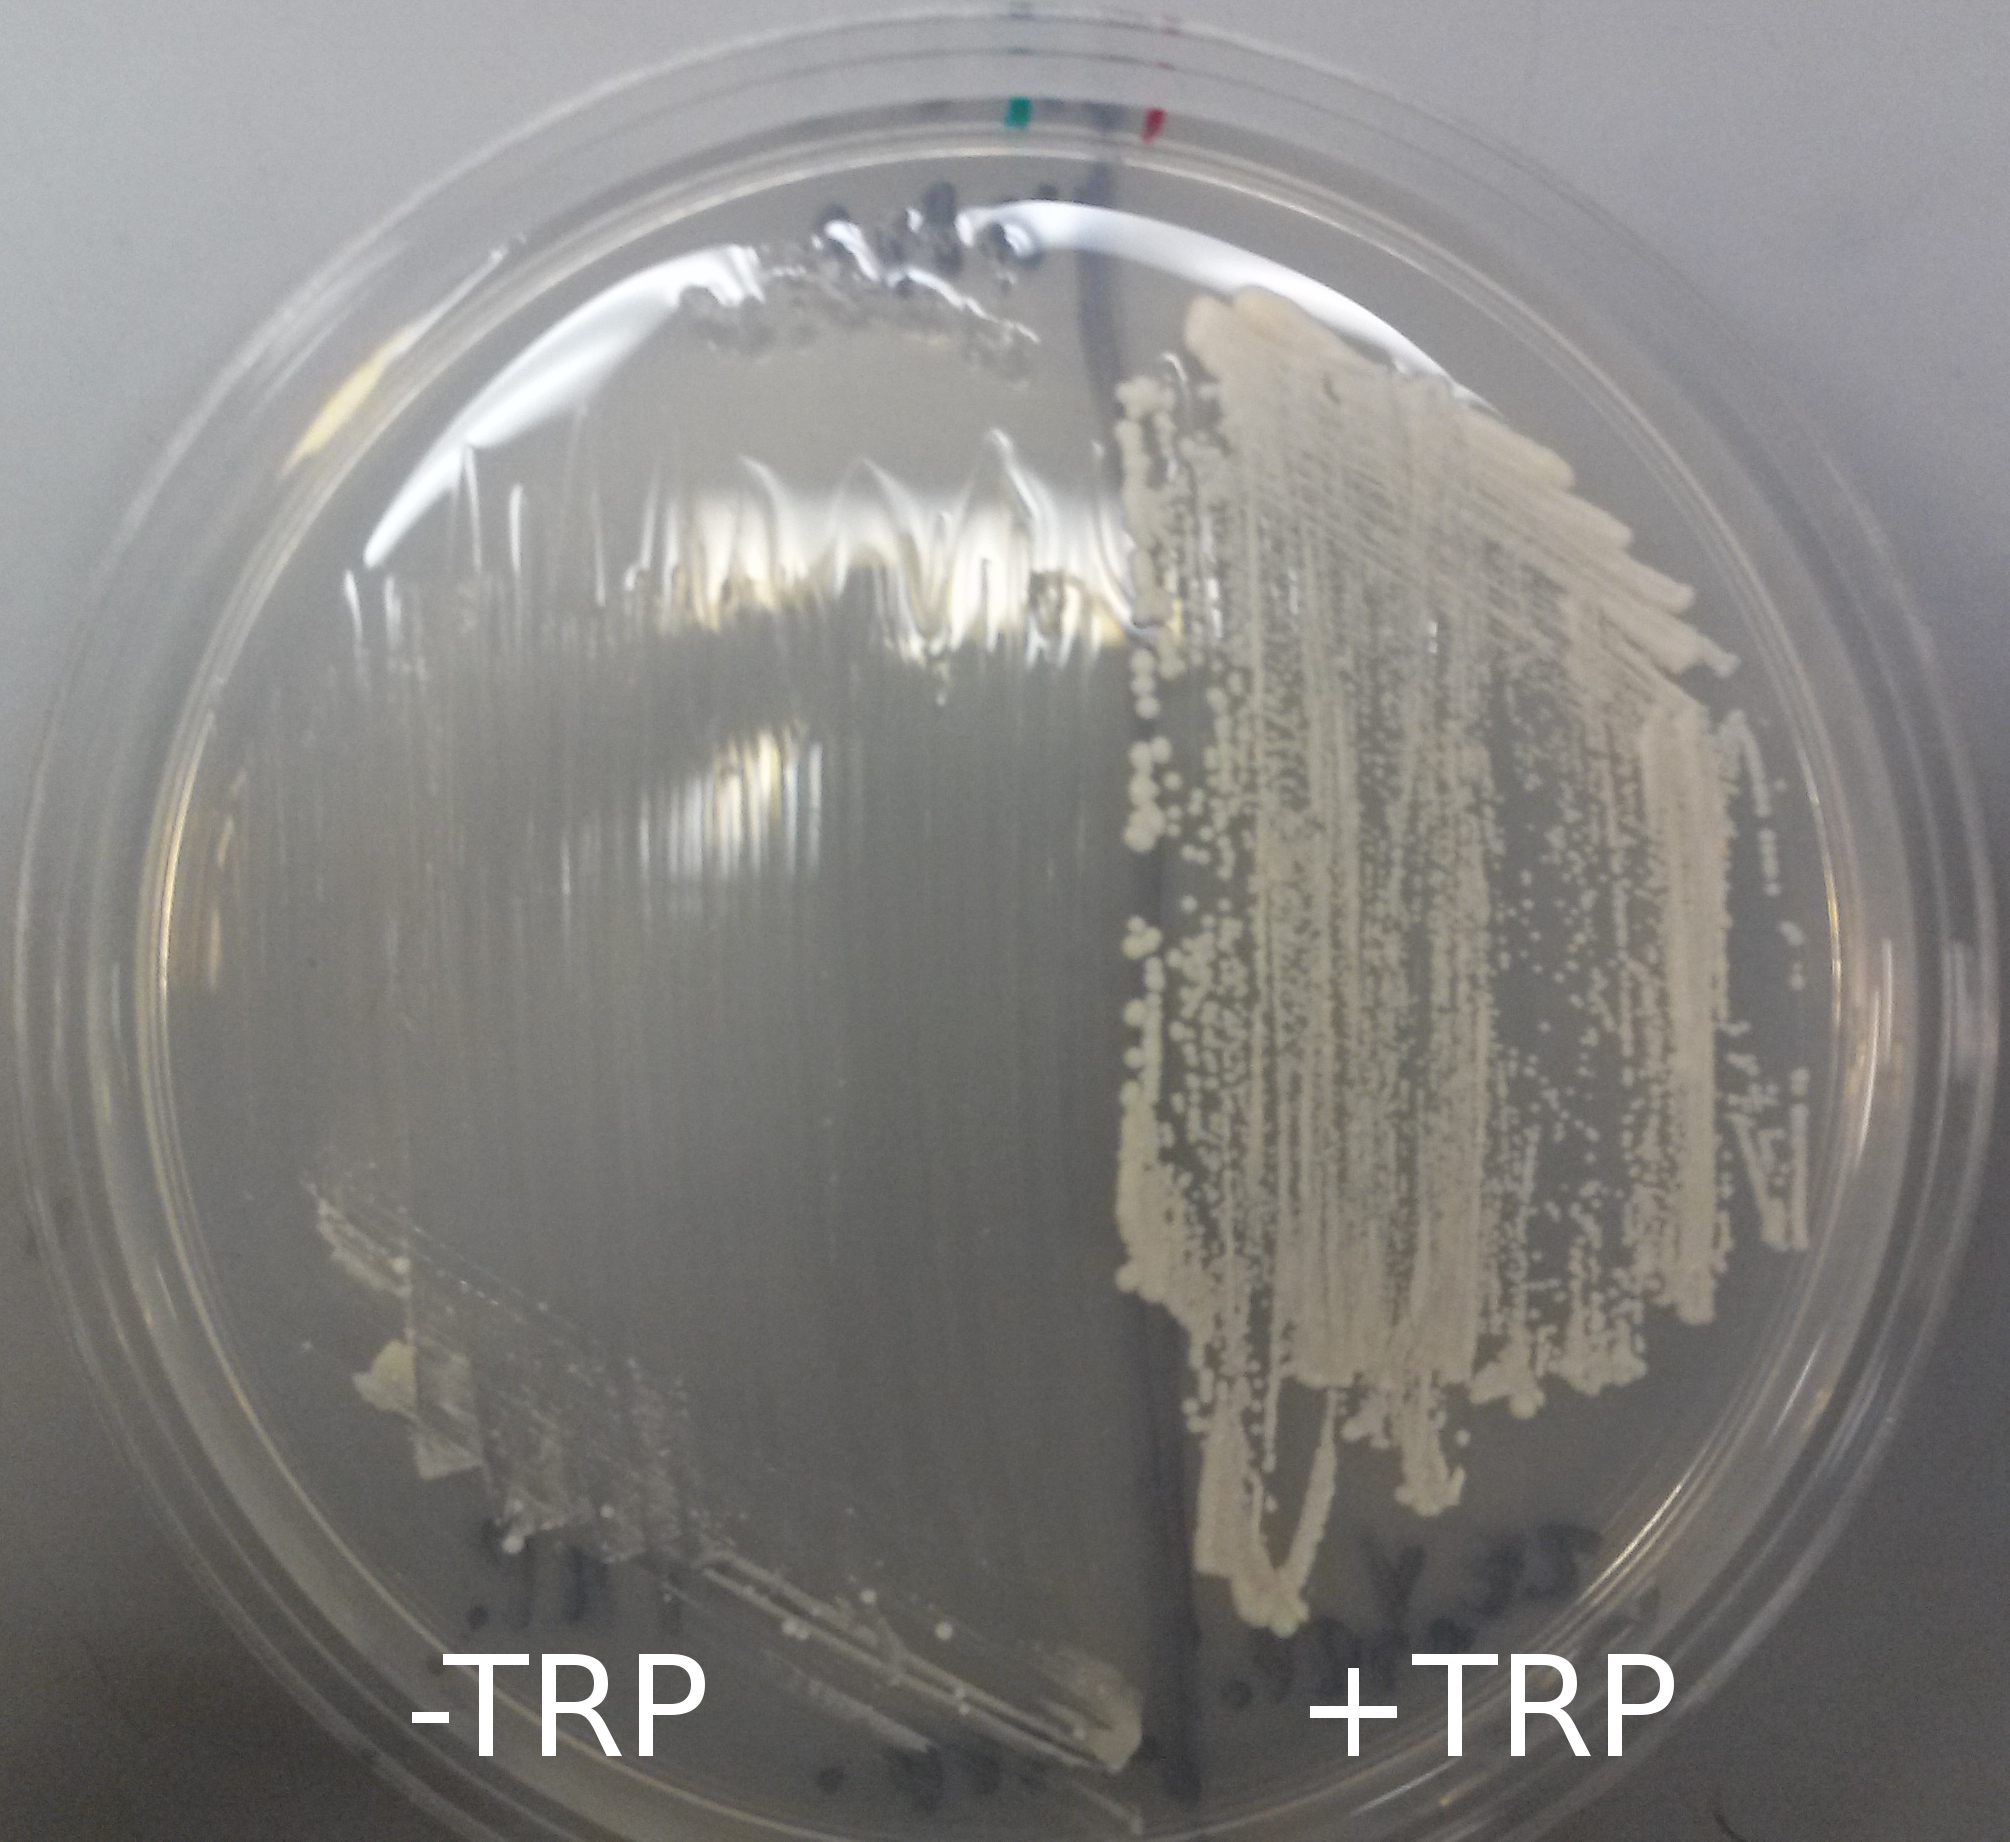
\includegraphics[width=.9\textwidth]{TRPtest.png}
            \caption{Test of SC -TRP plate}
            \label{fig:pcr}
        \end{figure}
    \end{minipage}

\end{frame}

\begin{frame}
   \begin{minipage}[ht!]{.48\textwidth}
          \begin{figure}[ht!]
            \centering
            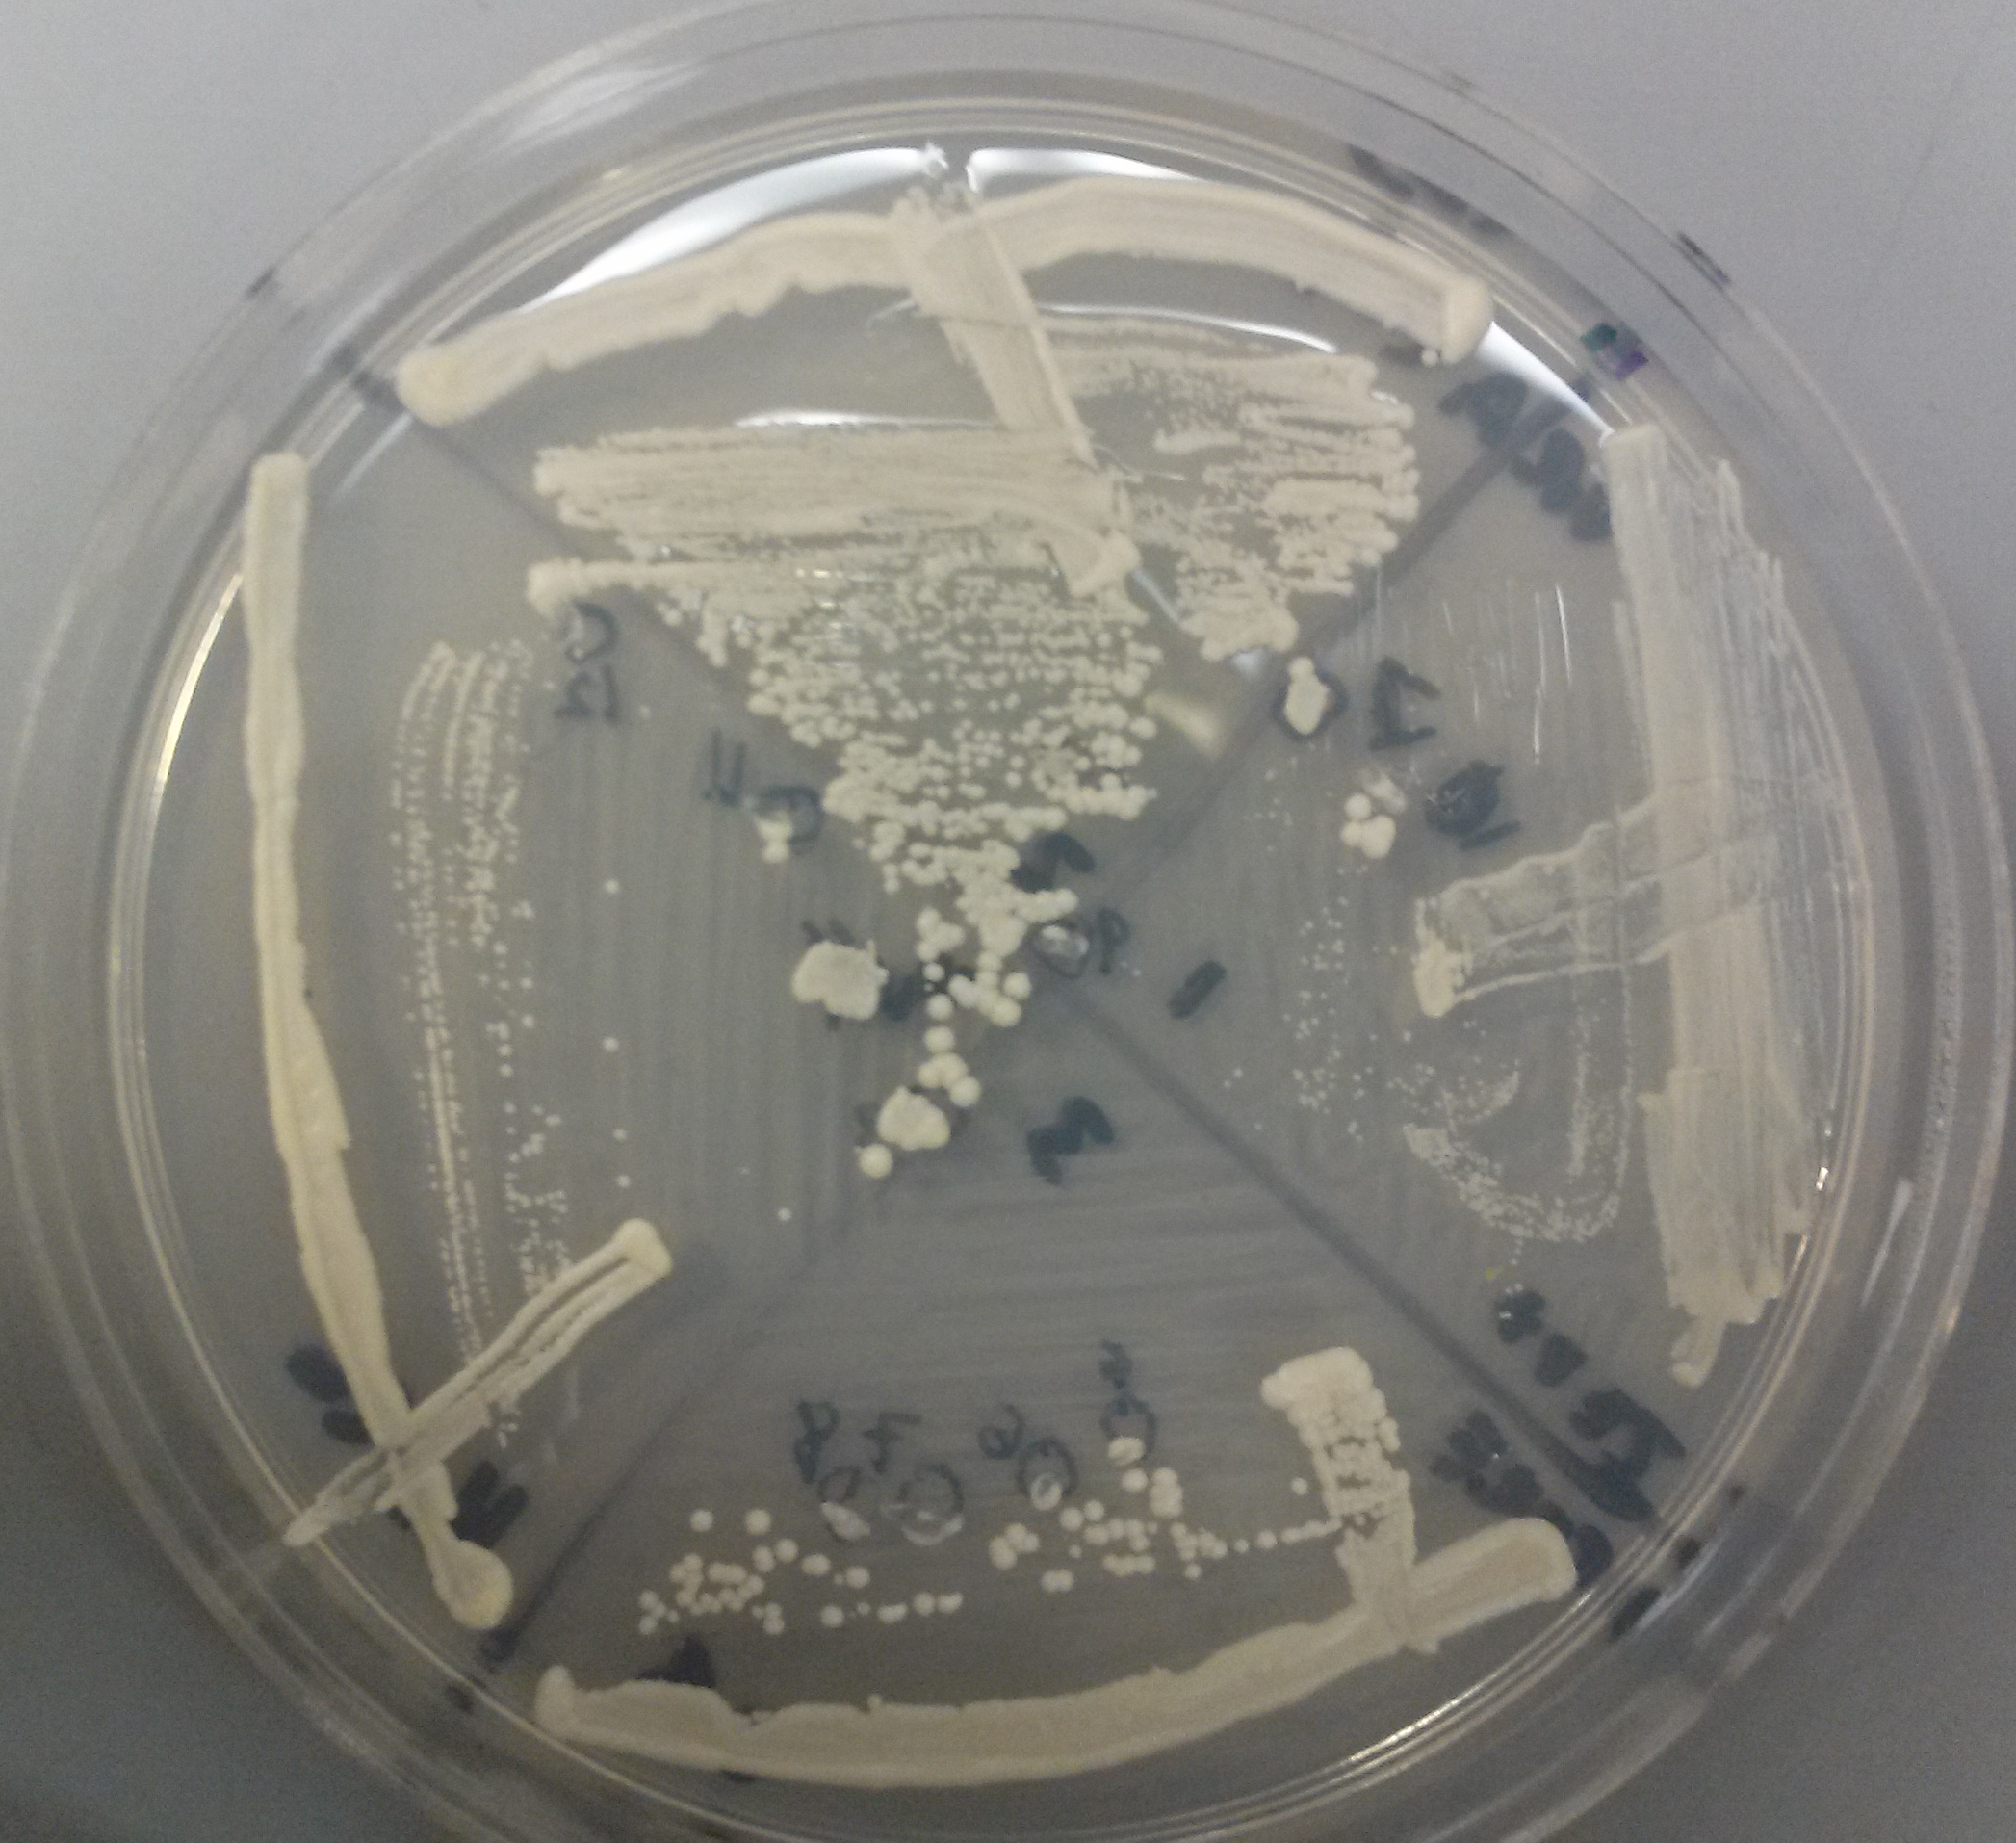
\includegraphics[width=.9\textwidth]{URArestreak1126.png}
            \label{fig:pcr}
        \end{figure}
    \end{minipage}
    \hfill
    \begin{minipage}[ht!]{.48\textwidth}
        \begin{itemize}
            \item<1-> Restreak transformants onto -URA from original G418.
            \item<2> Pick colonies to streak onto -TRP
        \end{itemize}
    \end{minipage}
\pause
 \begin{minipage}[ht!]{.48\textwidth}
          \begin{figure}[ht!]
            \centering
            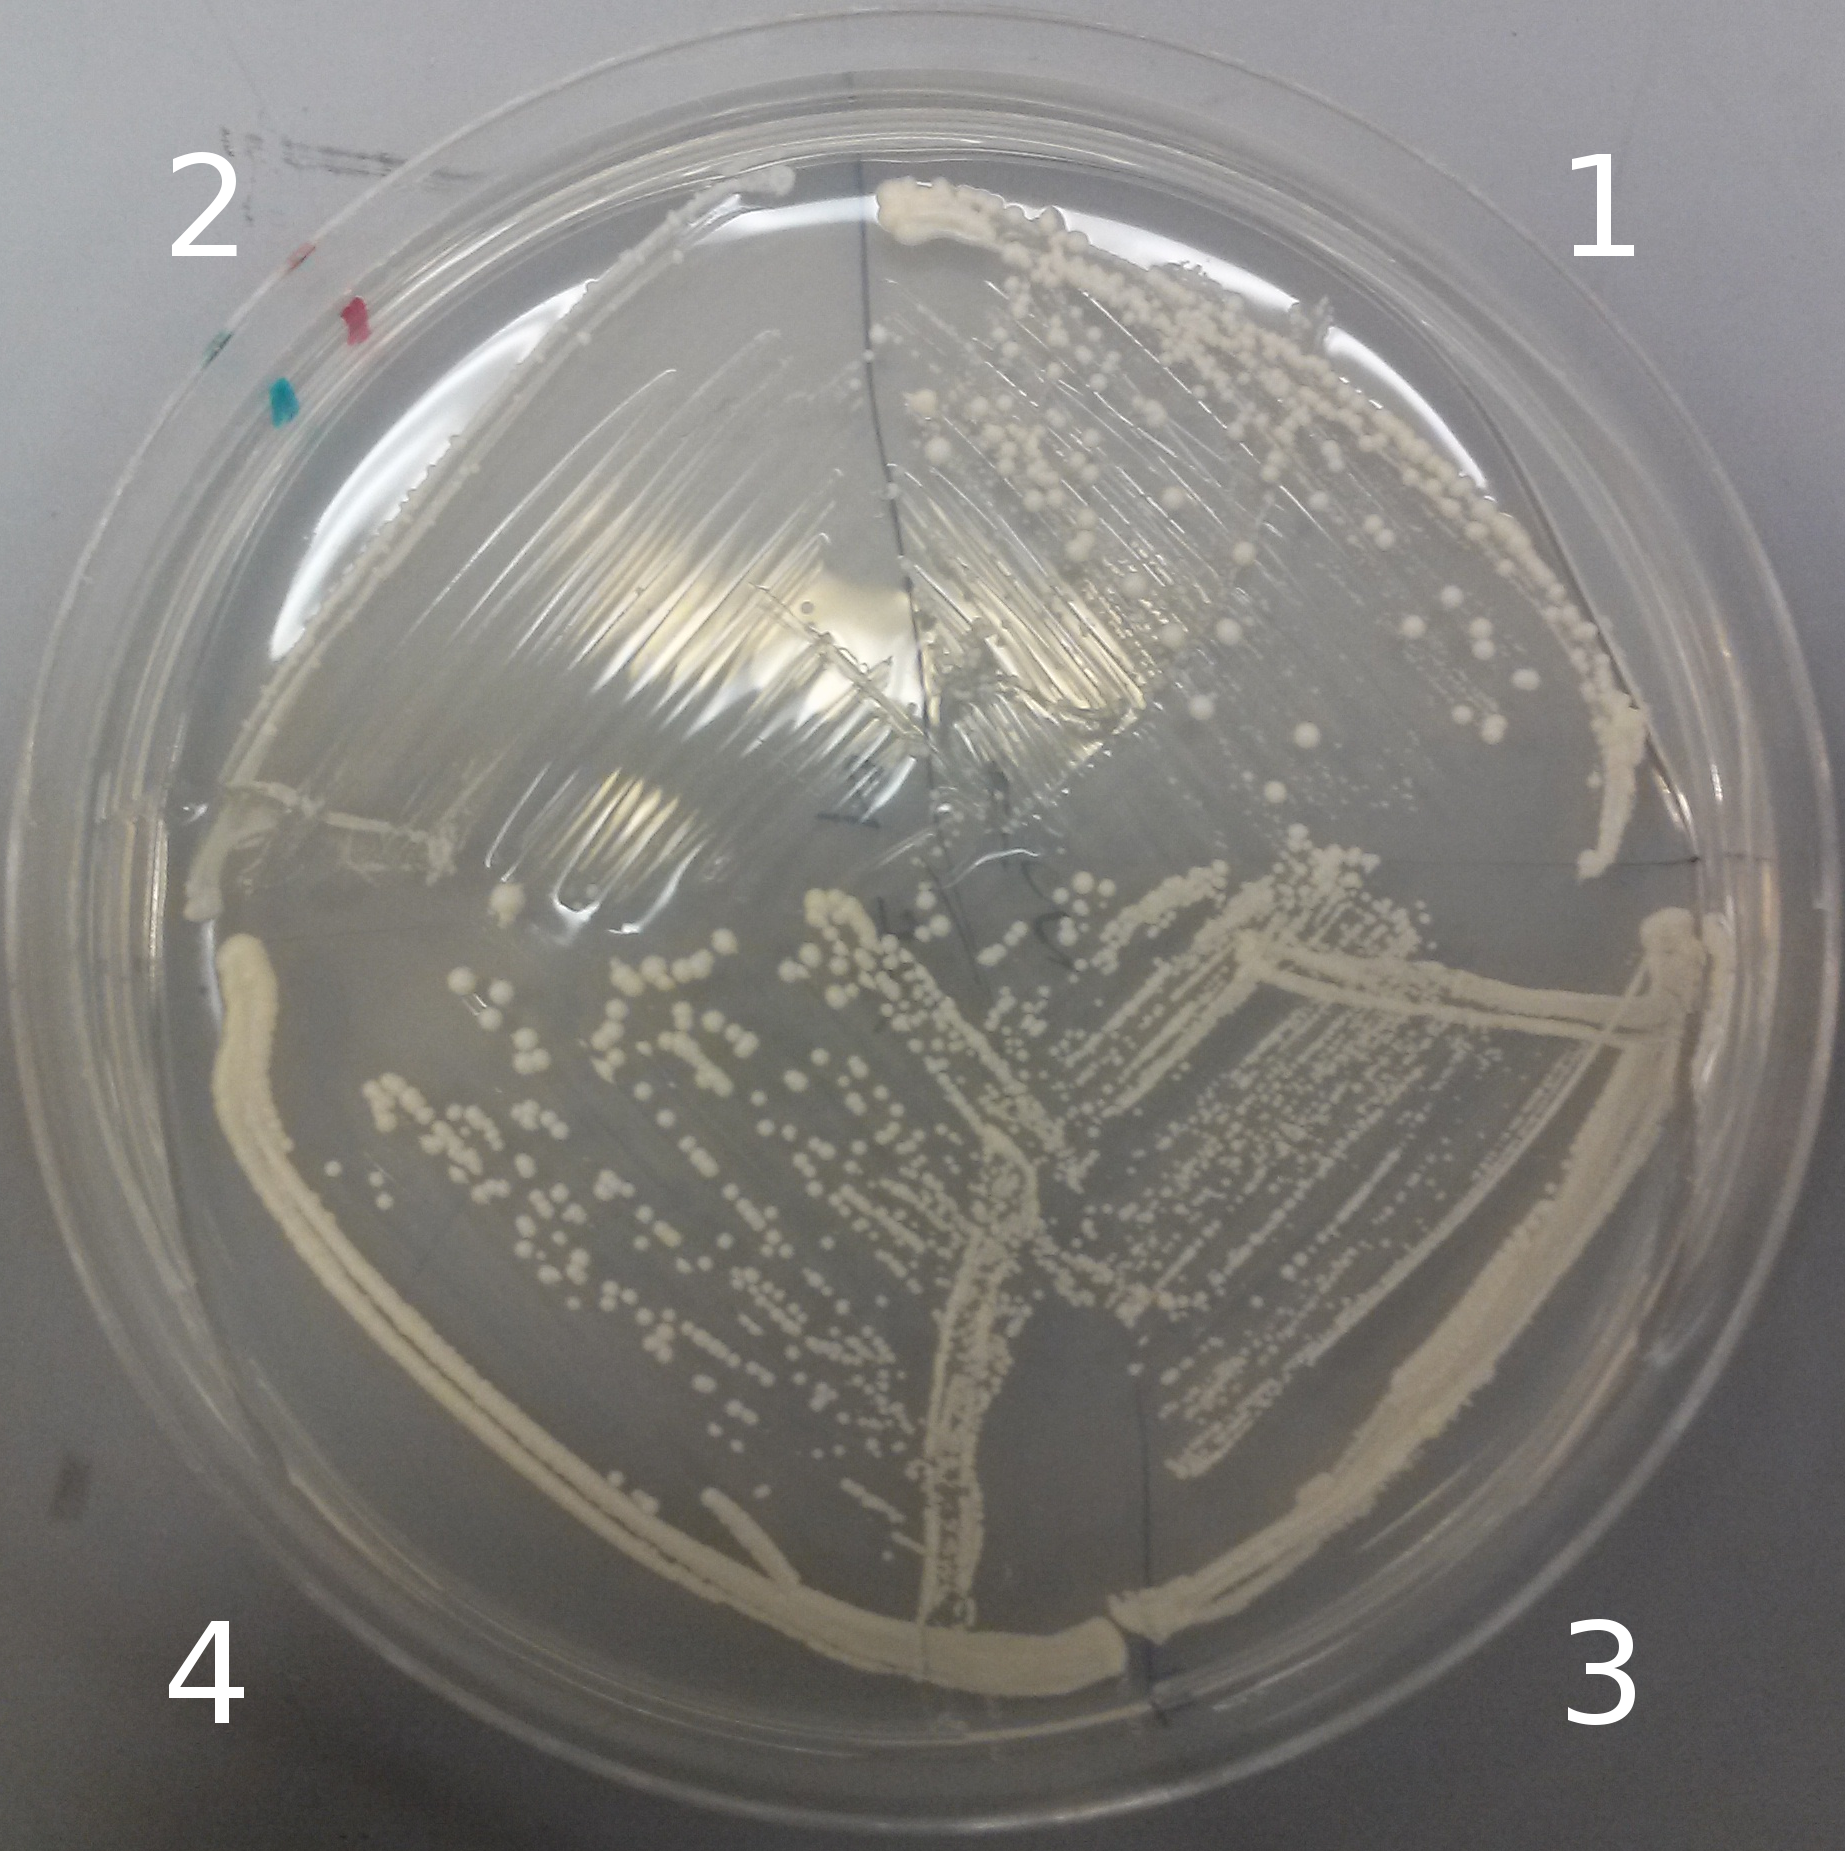
\includegraphics[width=.9\textwidth]{TRPrestreak1205a.png}
            \label{fig:pcr}
        \end{figure}
    \end{minipage}
    \hfill
    \begin{minipage}[ht!]{.48\textwidth}
         \begin{figure}[ht!]
            \centering
            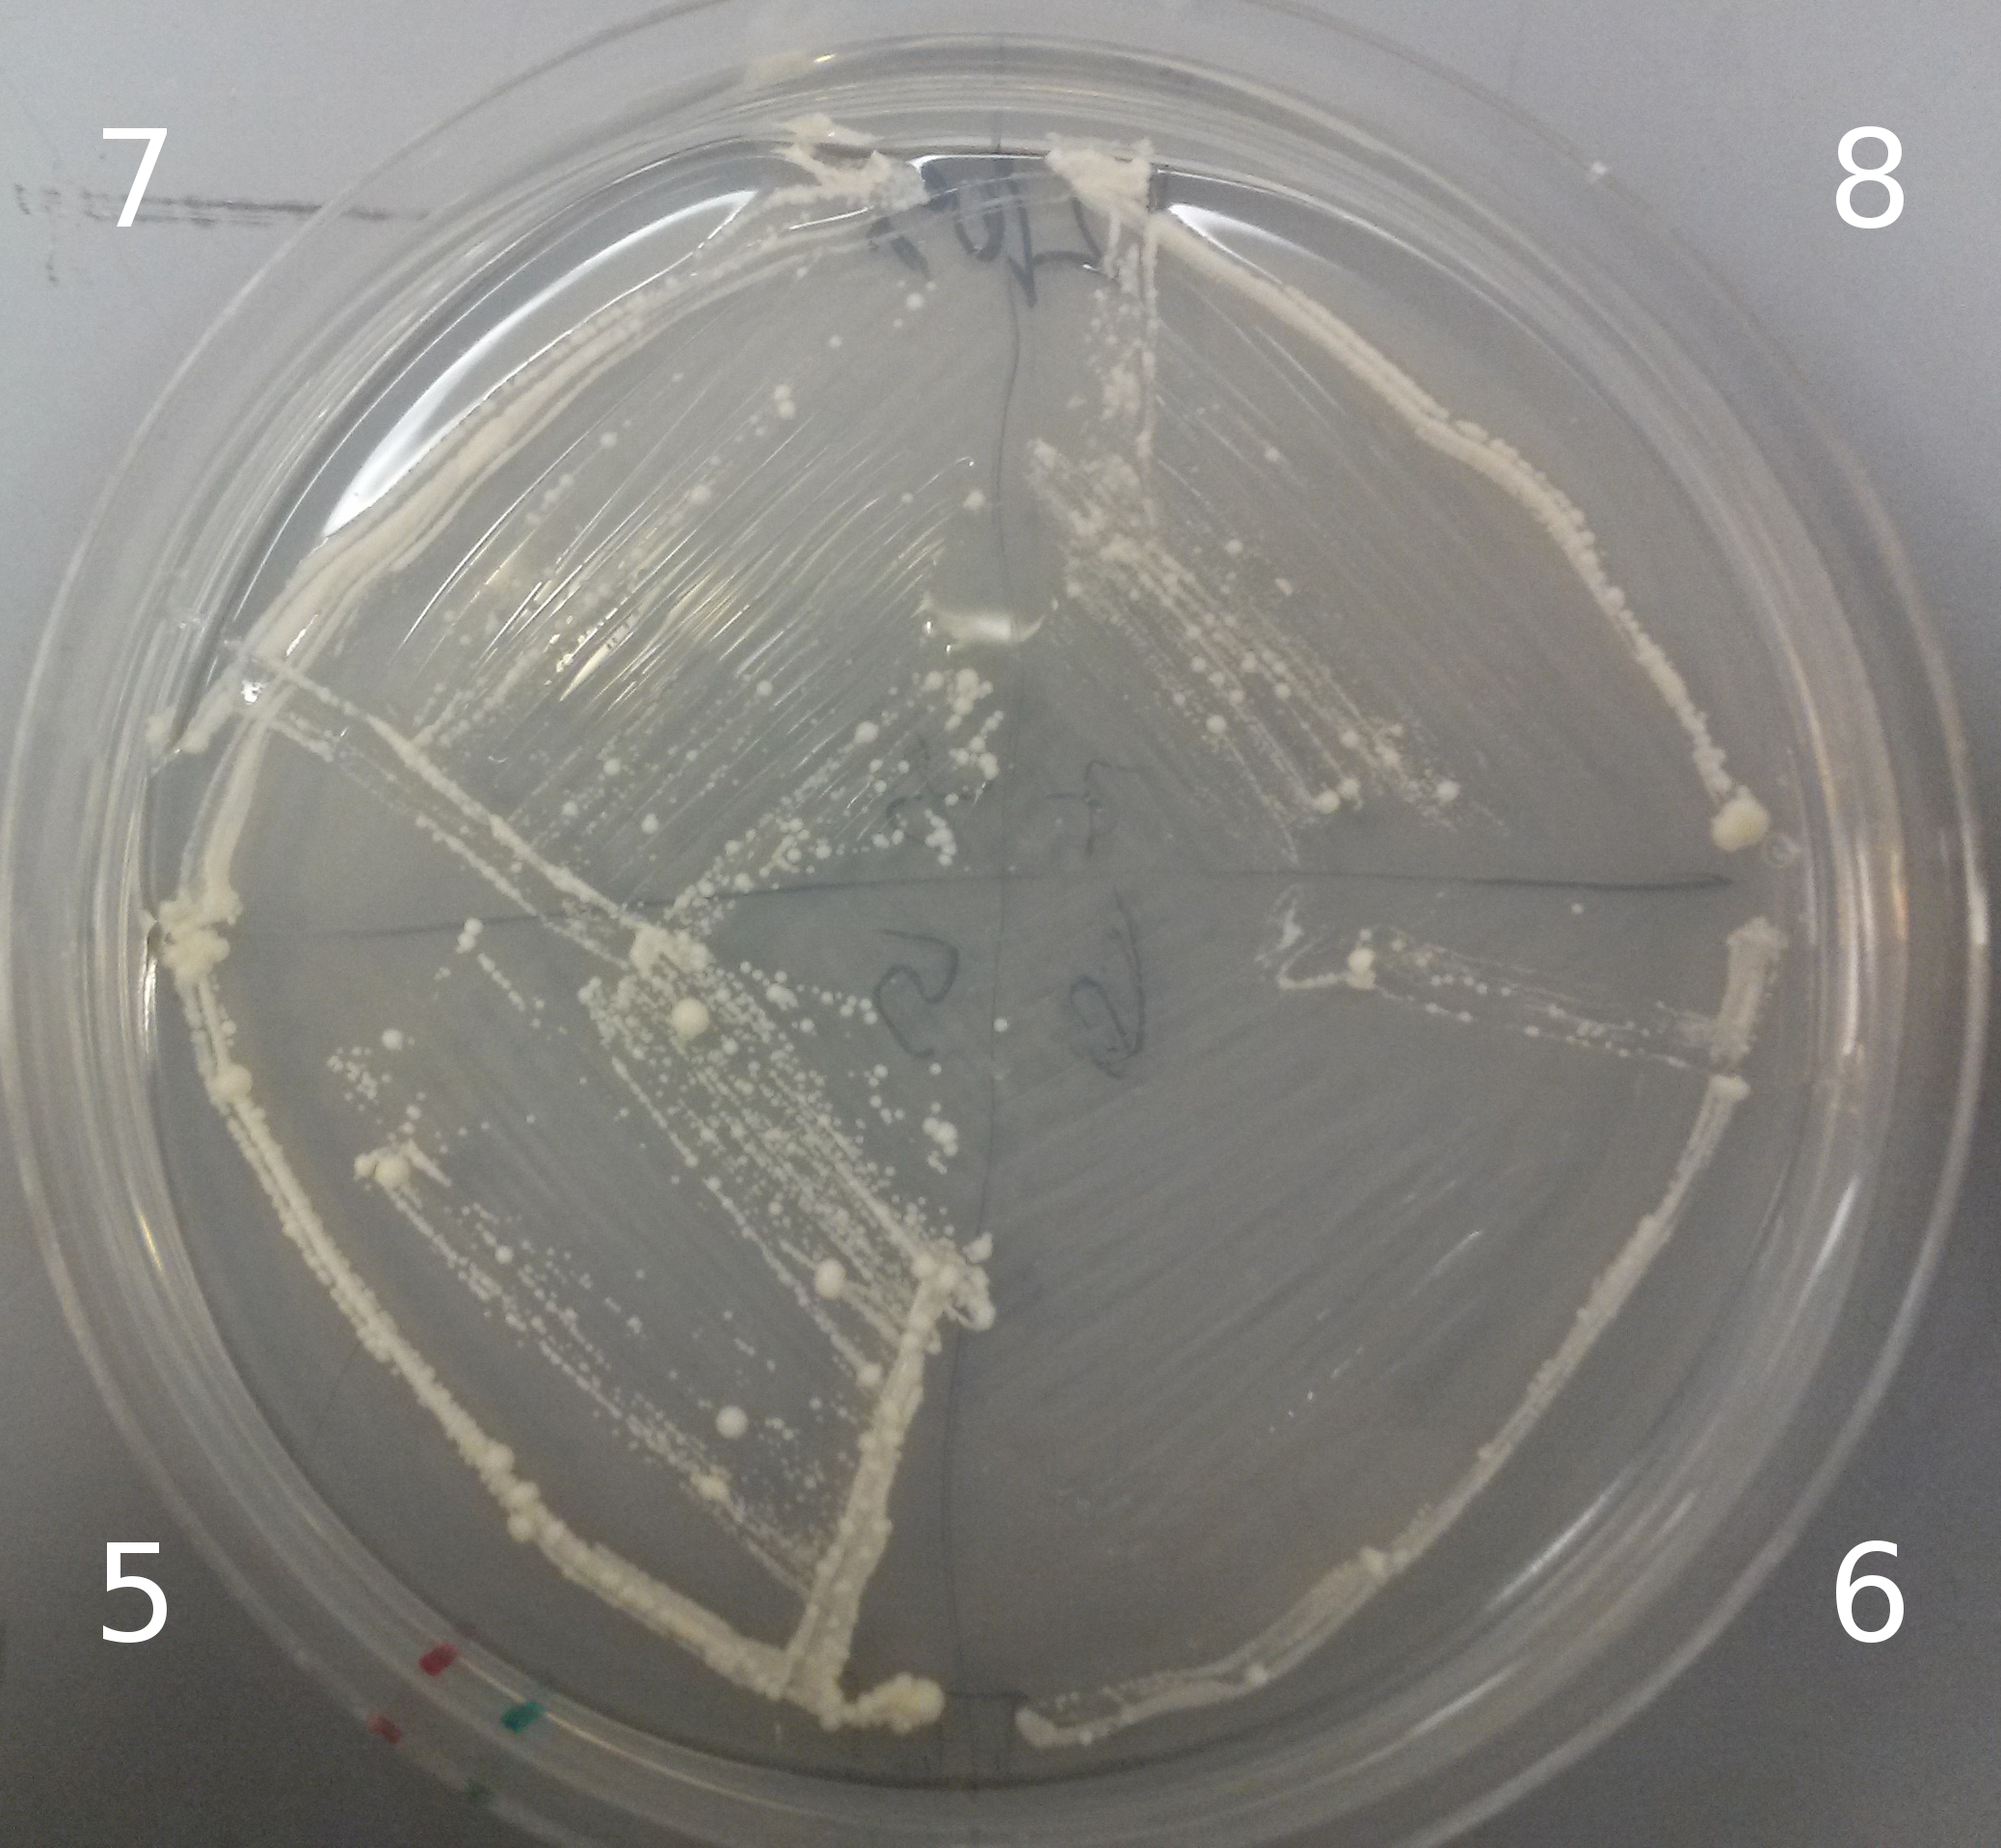
\includegraphics[width=.9\textwidth]{TRPrestreak1205b.png}
            \label{fig:pcr}
        \end{figure}
    \end{minipage}
\end{frame}



\begin{frame}
    \begin{itemize}
        \item Possibility: The CORE TRP KO fragment recombined with ClonNAT resistance.
        \item Replica plated onto G418+ClonNat; all colonies have G418+ClonNAT resistance.
            \pause
        \item Transformation of ZEV yeast w/ FAR + ZEVpr to knockout TRP directly.
    \end{itemize}
    \begin{figure}[ht!]
        \centering
        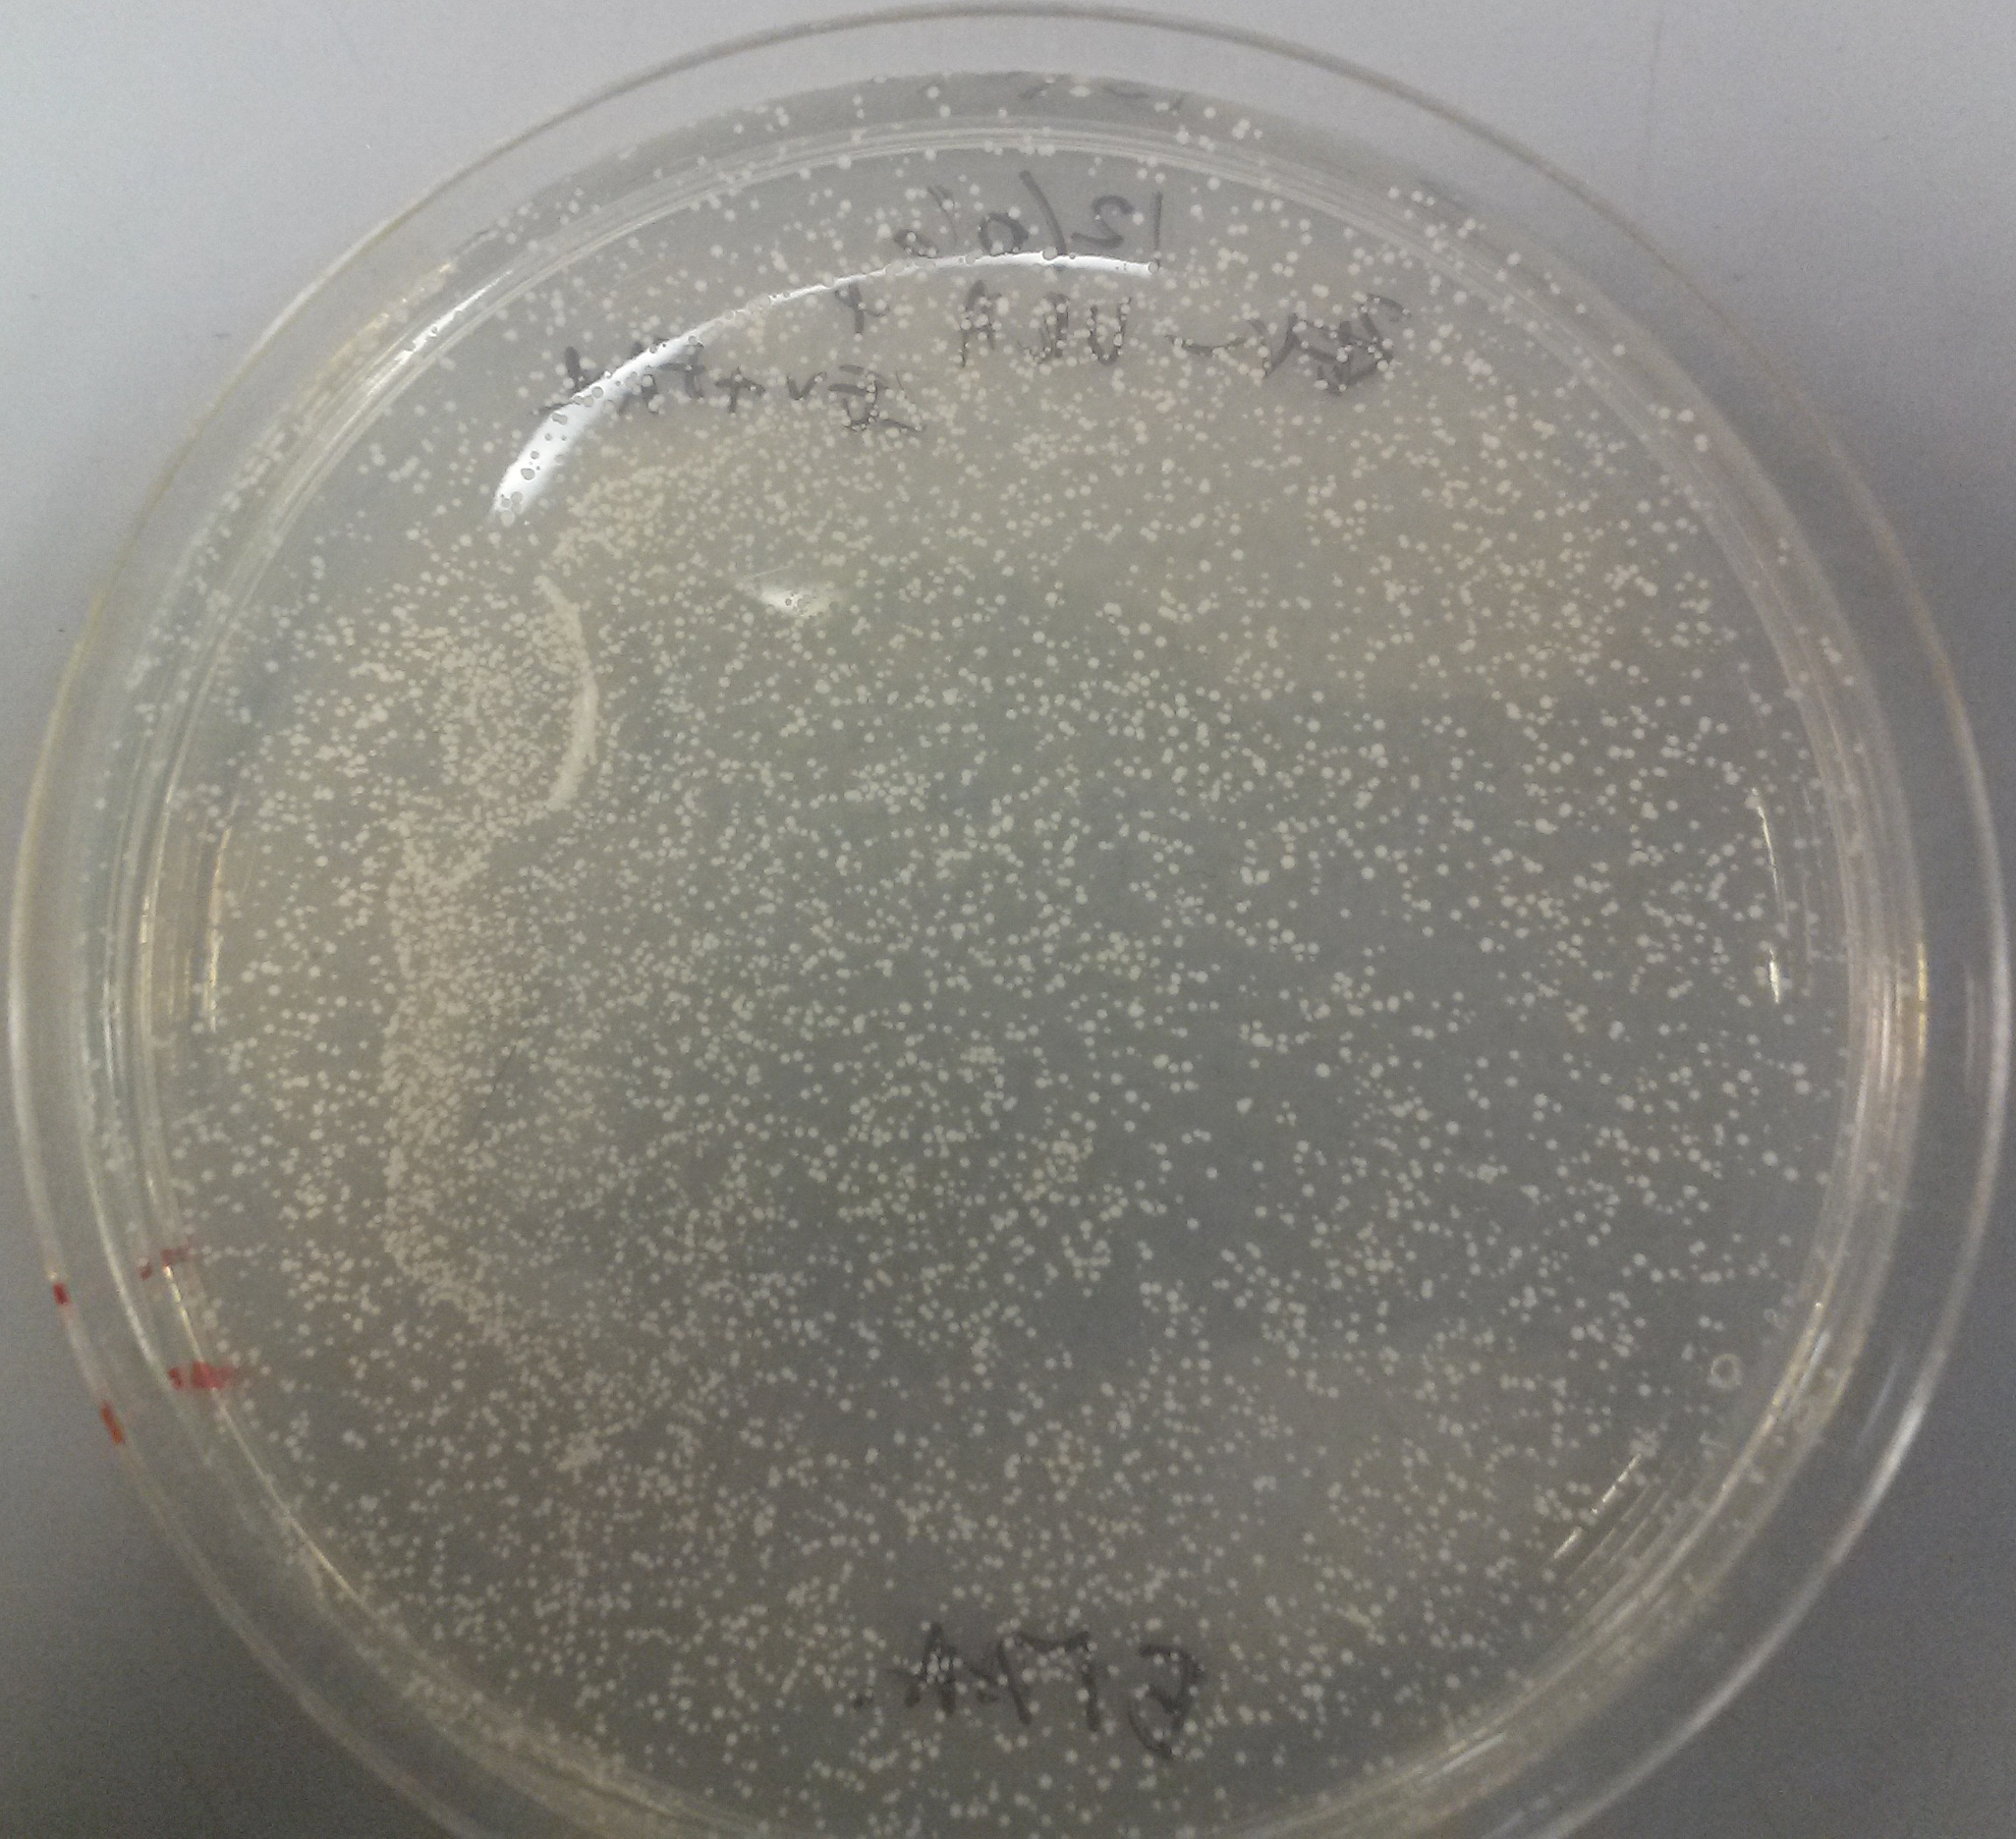
\includegraphics[width=.6\textwidth]{5FAA1206.png}
        \label{fig:faa}
    \end{figure}

\end{frame}

\begin{frame}
     \begin{center}
        {\large \textsc{Plasmid Construction:}}
    \end{center}
    Homologous recombination:
    \begin{figure}[ht!]
        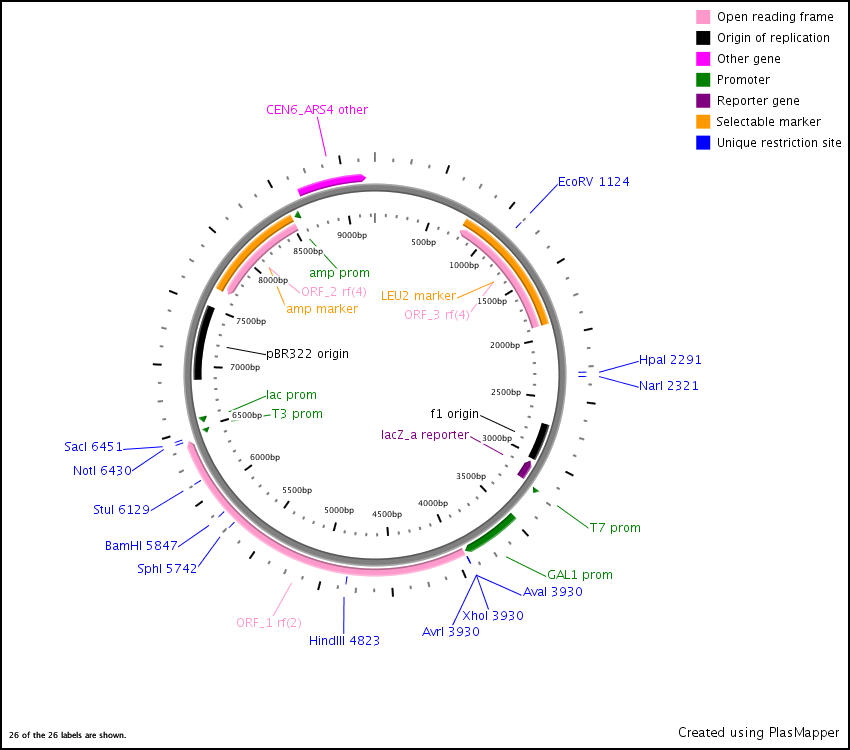
\includegraphics[width=.3\textwidth]{../Documents/plasMap_pGALFARwt.png}
        \label{fig:ligc}
    \end{figure}


    \begin{minipage}[ht!]{.48\textwidth}
          \begin{figure}[ht!]
            \centering
            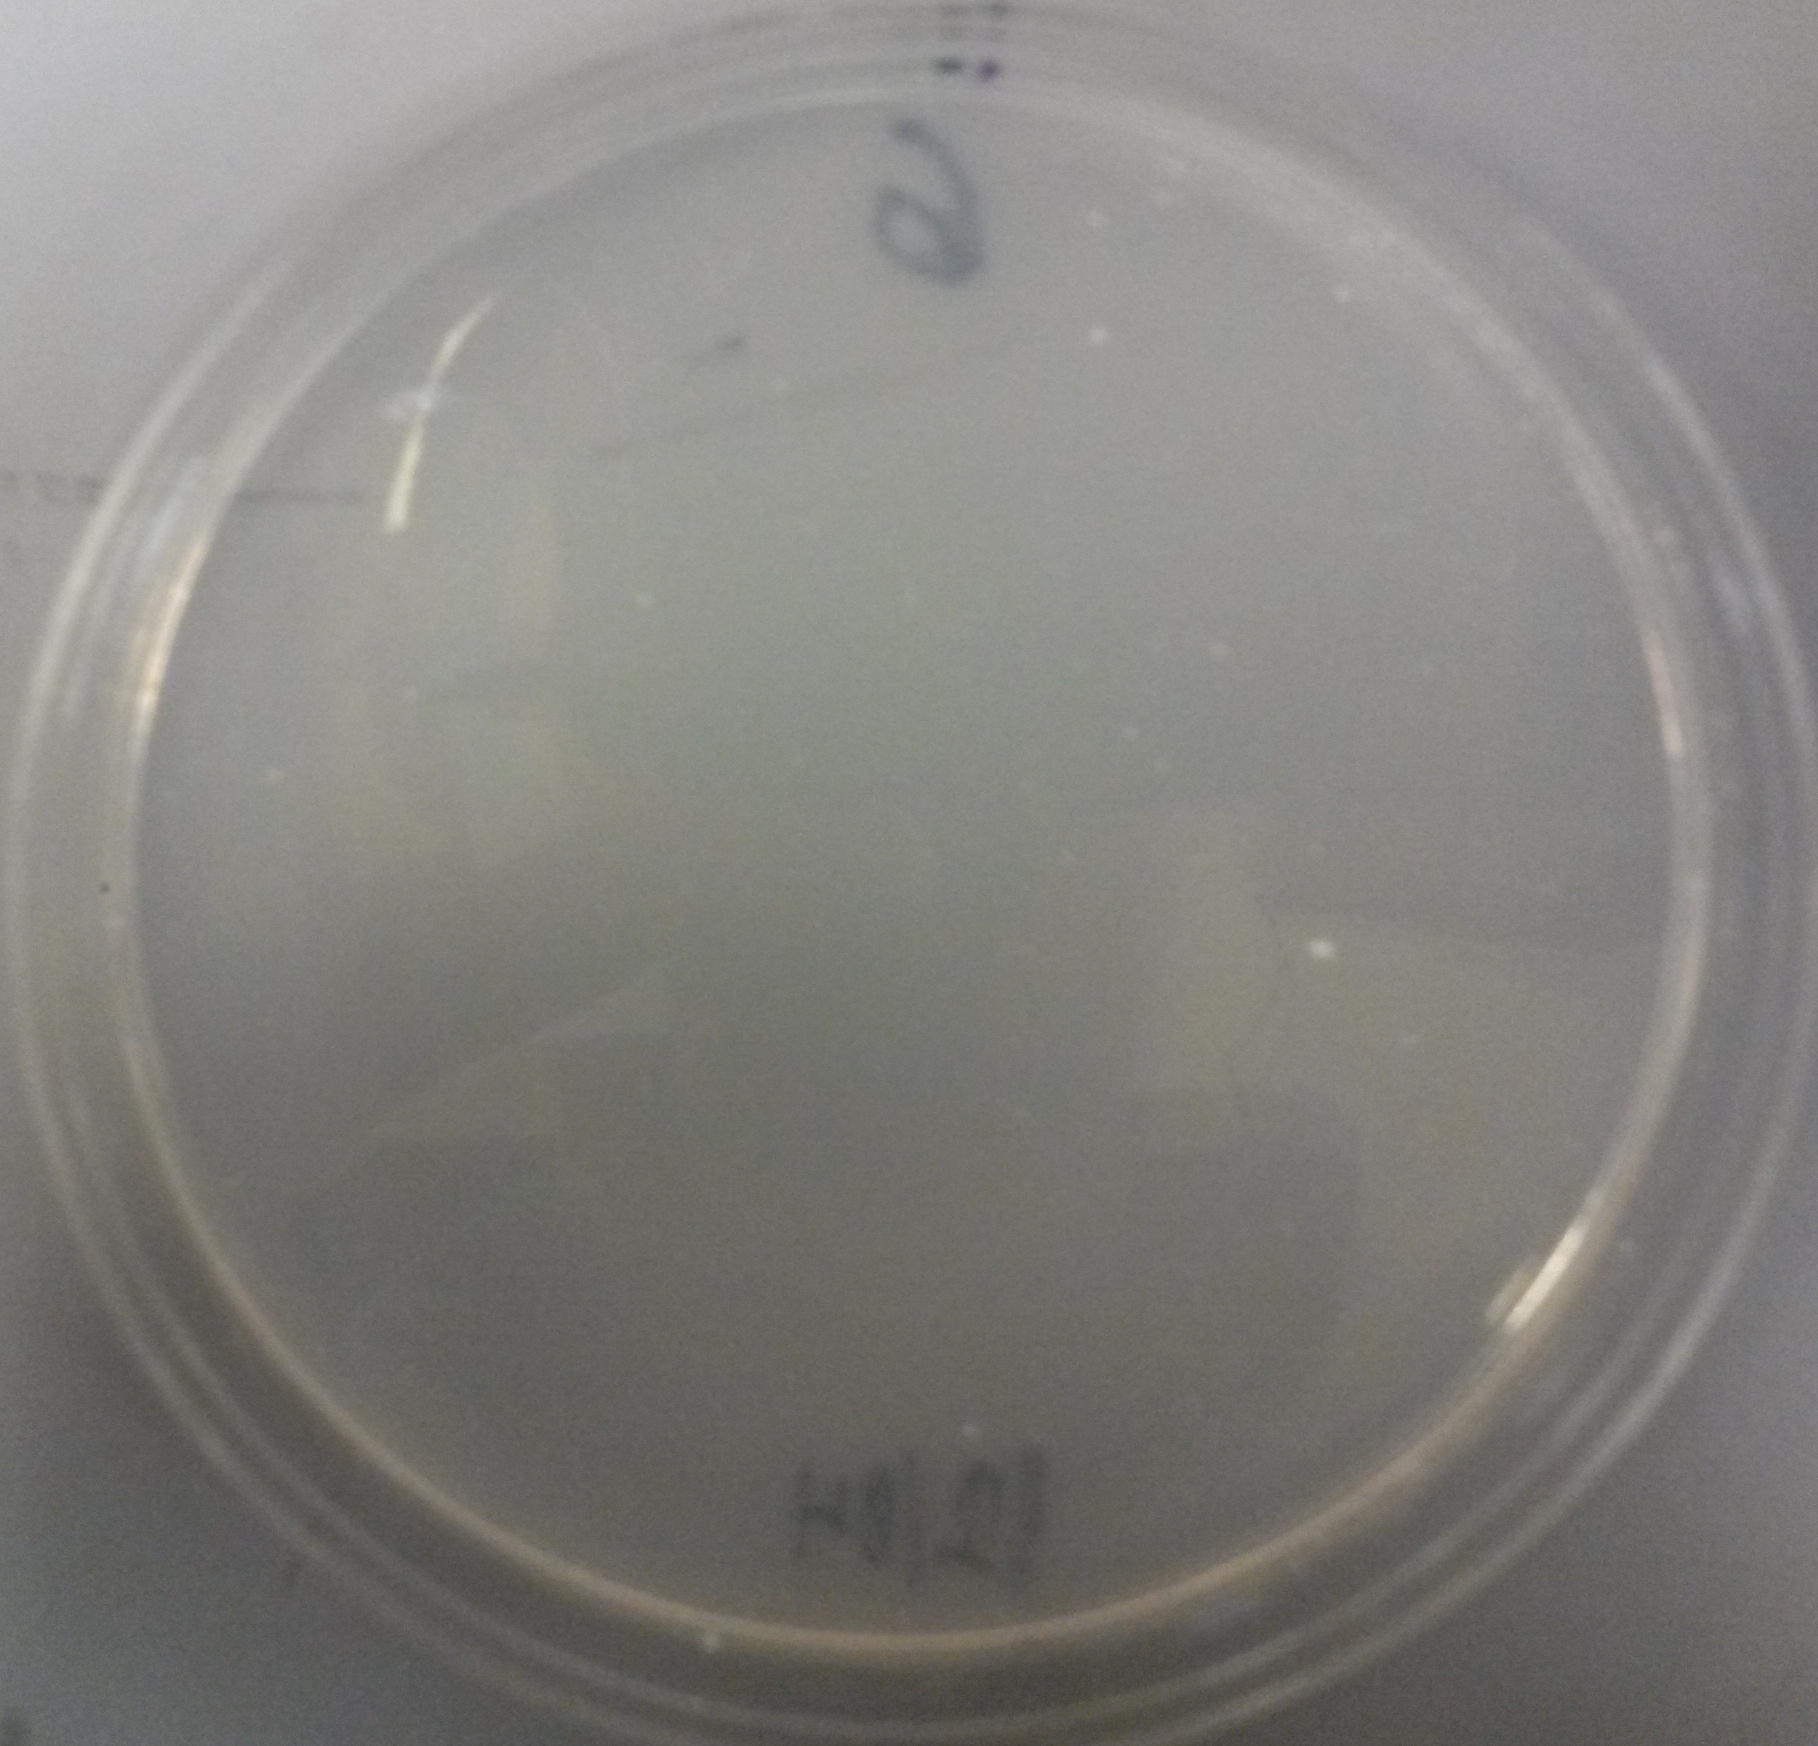
\includegraphics[width=.9\textwidth]{HRecomb1.png}
            \label{fig:pc2r}
            \caption{pGAL + FAR1-22}
        \end{figure}
    \end{minipage}
    \hfill
    \begin{minipage}[ht!]{.48\textwidth}
         \begin{figure}[ht!]
            \centering
            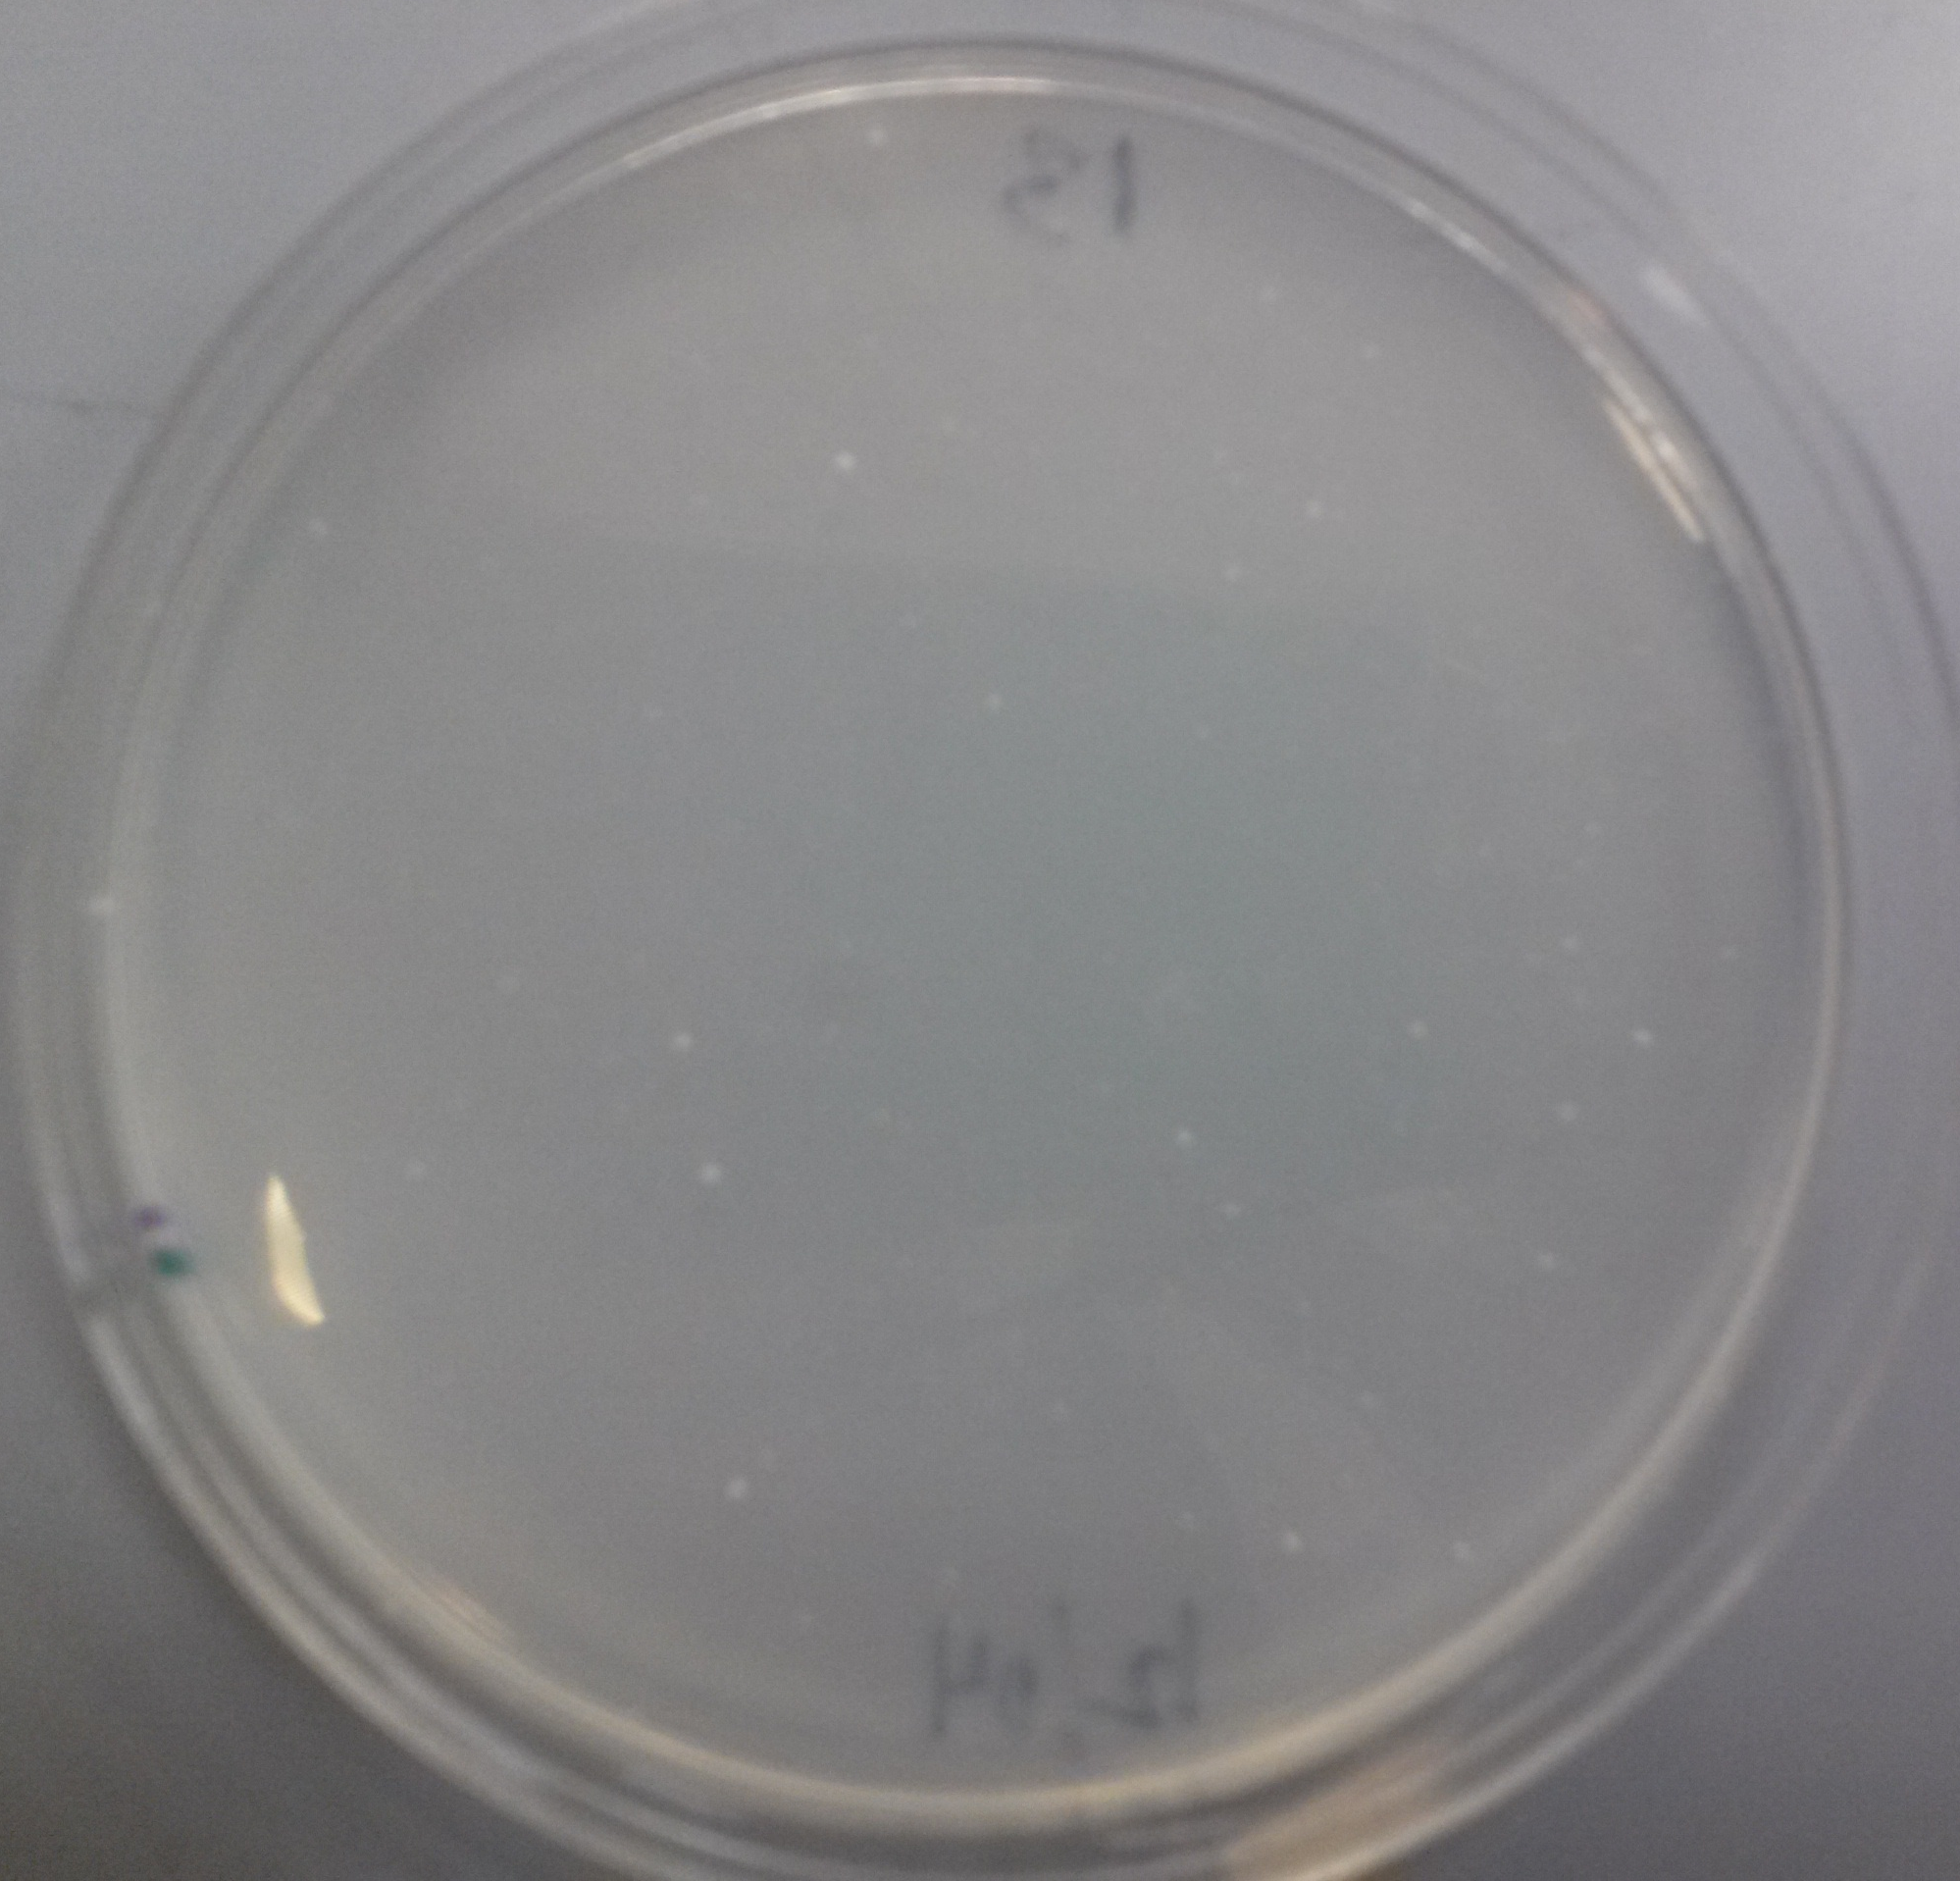
\includegraphics[width=.9\textwidth]{HRecomb2.png}
            \caption{pGAL + FAR1-WT}
            \label{fig:pc3r}
        \end{figure}
    \end{minipage}
\end{frame}

\begin{frame}
    \begin{itemize}
        \item \textbf{Backup:} Transform the plasmid that we know to contain FAR1-22 under the GAL promoter into a \emph{-HIS} strain
    \end{itemize}
    \begin{figure}[ht!]
        \centering
        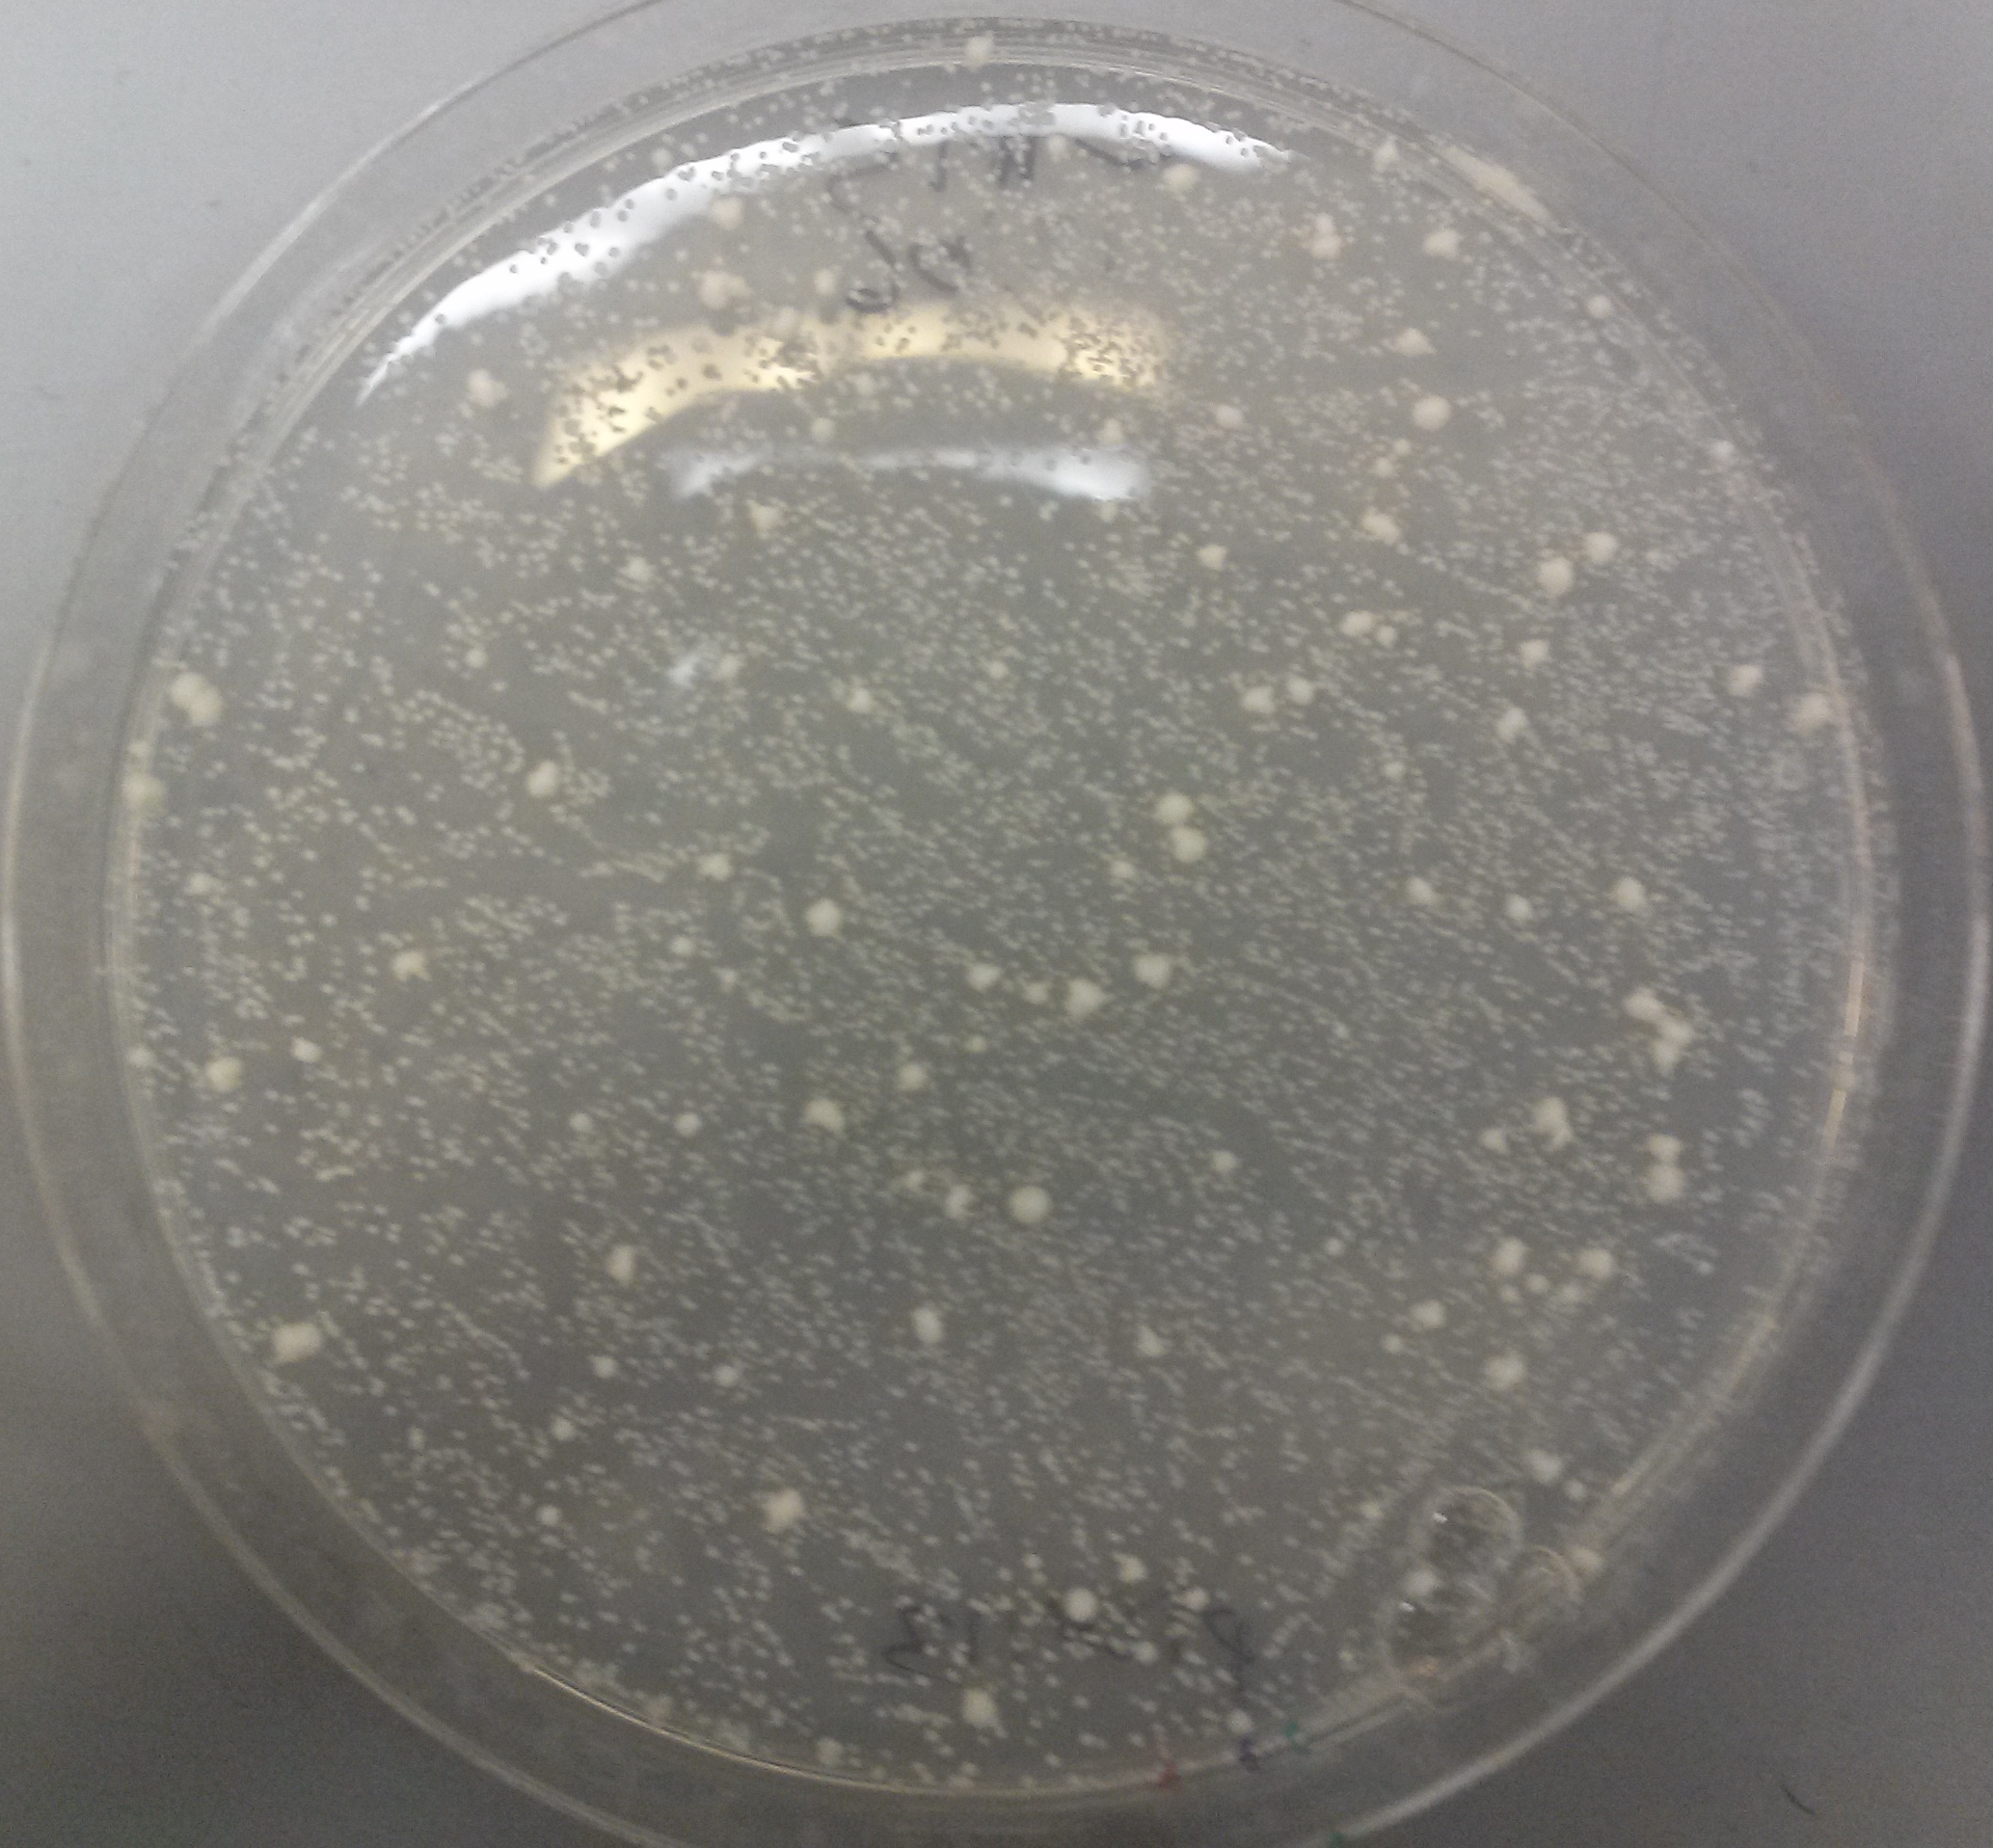
\includegraphics[width=.6\textwidth]{HIS1206.png}
        \label{fig:faa}
    \end{figure}
\end{frame}

\begin{frame}
    \begin{center}
        {\large \textsc{This week (12/09) and next?}}
    \end{center}
    \textbf{Test pGAL + FAR1-22:}\\
    \begin{itemize}
        \item Raffinose starvation.
        \item Glucose/Galactose gradient.
        \item FACS experiments with DNA dye (against untransformed -HIS strain)
            \bigskip
        \item Continue construction of pGAL + FAR1-22 and pGAL + FAR1-WT.
    \end{itemize}
\end{frame}

\begin{frame}
    \textbf{Today!}

    \begin{itemize}
        \item Colony PCR colonies from 5-FAA plate to confirm TRP KO. (Will use primers for ZEVpr fragment, which is smaller).
            \bigskip
        \item PCR of ZEVpr, FAR1-22, and \textbf{FAR1-WT} to do genomic construction by 5-FAA again.
            \bigskip
        \item Set up raffinose starvation tomorrow.
        \item Set up galactose/glucose media. Dilutions + plates.
    \end{itemize}
\end{frame}

\end{document}
